\documentclass[border={20.000000bp 20.000000bp 20.000000bp 20.000000bp}, 11pt]{standalone}
\pdfinfoomitdate=1
\pdftrailerid{}
\pdfsuppressptexinfo=1
\pdfinfo{ /Creator () /Producer () }

\usepackage{tikz}
\usepackage{xcolor}
\usetikzlibrary{shapes.misc}
\usetikzlibrary{backgrounds}

\definecolor{dotColorA}{HTML}{000000}
\definecolor{dotColorB}{HTML}{000000}
\definecolor{dotColorC}{HTML}{000000}
\definecolor{dotColorD}{HTML}{000000}
\definecolor{dotColorE}{HTML}{000000}
\definecolor{dotColorF}{HTML}{000000}
\definecolor{dotColorG}{HTML}{000000}
\definecolor{dotColorH}{HTML}{000000}
\definecolor{dotColorI}{HTML}{000000}
\definecolor{dotColorJ}{HTML}{000000}
\definecolor{dotColorK}{HTML}{000000}
\definecolor{dotColorL}{HTML}{000000}
\definecolor{dotColorM}{HTML}{000000}
\definecolor{dotColorN}{HTML}{000000}
\definecolor{dotColorO}{HTML}{000000}

\definecolor{labelBgColorA}{HTML}{1F77B4}
\definecolor{labelBgColorB}{HTML}{FF7F0E}
\definecolor{labelBgColorC}{HTML}{2CA02C}
\definecolor{labelBgColorD}{HTML}{D62728}
\definecolor{labelBgColorE}{HTML}{9467BD}
\definecolor{labelBgColorF}{HTML}{8C564B}
\definecolor{labelBgColorG}{HTML}{E377C2}
\definecolor{labelBgColorH}{HTML}{7F7F7F}
\definecolor{labelBgColorI}{HTML}{BCBD22}
\definecolor{labelBgColorJ}{HTML}{17BECF}
\definecolor{labelBgColorK}{HTML}{1F77B4}
\definecolor{labelBgColorL}{HTML}{FF7F0E}
\definecolor{labelBgColorM}{HTML}{2CA02C}
\definecolor{labelBgColorN}{HTML}{D62728}
\definecolor{labelBgColorO}{HTML}{9467BD}

\definecolor{labelTextColorA}{HTML}{FFFFFF}
\definecolor{labelTextColorB}{HTML}{FFFFFF}
\definecolor{labelTextColorC}{HTML}{FFFFFF}
\definecolor{labelTextColorD}{HTML}{FFFFFF}
\definecolor{labelTextColorE}{HTML}{FFFFFF}
\definecolor{labelTextColorF}{HTML}{FFFFFF}
\definecolor{labelTextColorG}{HTML}{FFFFFF}
\definecolor{labelTextColorH}{HTML}{FFFFFF}
\definecolor{labelTextColorI}{HTML}{FFFFFF}
\definecolor{labelTextColorJ}{HTML}{FFFFFF}
\definecolor{labelTextColorK}{HTML}{FFFFFF}
\definecolor{labelTextColorL}{HTML}{FFFFFF}
\definecolor{labelTextColorM}{HTML}{FFFFFF}
\definecolor{labelTextColorN}{HTML}{FFFFFF}
\definecolor{labelTextColorO}{HTML}{FFFFFF}

\definecolor{linkColorA}{HTML}{1F77B4}
\definecolor{linkColorB}{HTML}{FF7F0E}
\definecolor{linkColorC}{HTML}{2CA02C}
\definecolor{linkColorD}{HTML}{D62728}
\definecolor{linkColorE}{HTML}{9467BD}
\definecolor{linkColorF}{HTML}{8C564B}
\definecolor{linkColorG}{HTML}{E377C2}
\definecolor{linkColorH}{HTML}{7F7F7F}
\definecolor{linkColorI}{HTML}{BCBD22}
\definecolor{linkColorJ}{HTML}{17BECF}
\definecolor{linkColorK}{HTML}{1F77B4}
\definecolor{linkColorL}{HTML}{FF7F0E}
\definecolor{linkColorM}{HTML}{2CA02C}
\definecolor{linkColorN}{HTML}{D62728}
\definecolor{linkColorO}{HTML}{9467BD}


\begin{document}
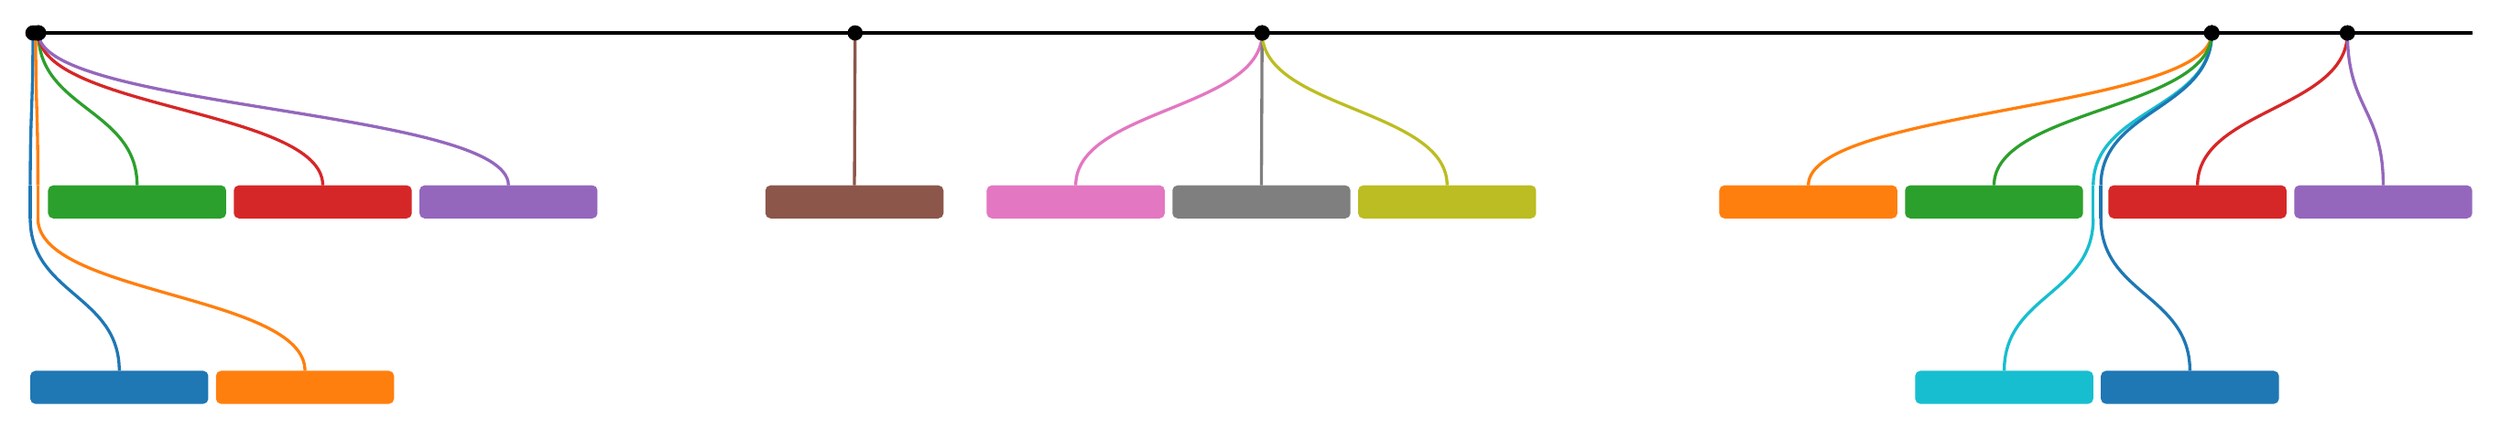
\begin{tikzpicture}[x=1bp,y=-1bp]

% shift for the margin
\begin{scope}[shift={(20, 20)}]
% main layer
\begin{scope}[shift={(0, 0)}]
% axis
\begin{scope}
\draw[very thick] (0, 0) -- (960, 0);
\end{scope}

% link layer
\begin{scope}
\draw[color=linkColorA, very thick] (1.06666667, 0.00000000) .. controls
(1.06666667, 30.00000000) and (0.00000000, 30.00000000) .. (0.00000000, 60.00000000);
\draw[color=linkColorA, very thick] (0.00000000, 60.00000000) -- (0.00000000, 73.00000000);
\draw[color=linkColorA, very thick] (0.00000000, 73.00000000) .. controls
(0.00000000, 103.00000000) and (35.00000000, 103.00000000) .. (35.00000000, 133.00000000);
\draw[color=linkColorB, very thick] (2.13333333, 0.00000000) .. controls
(2.13333333, 30.00000000) and (3.00000000, 30.00000000) .. (3.00000000, 60.00000000);
\draw[color=linkColorB, very thick] (3.00000000, 60.00000000) -- (3.00000000, 73.00000000);
\draw[color=linkColorB, very thick] (3.00000000, 73.00000000) .. controls
(3.00000000, 103.00000000) and (108.00000000, 103.00000000) .. (108.00000000, 133.00000000);
\draw[color=linkColorC, very thick] (3.20000000, 0.00000000) .. controls
(3.20000000, 30.00000000) and (42.00000000, 30.00000000) .. (42.00000000, 60.00000000);
\draw[color=linkColorD, very thick] (3.20000000, 0.00000000) .. controls
(3.20000000, 30.00000000) and (115.00000000, 30.00000000) .. (115.00000000, 60.00000000);
\draw[color=linkColorE, very thick] (3.20000000, 0.00000000) .. controls
(3.20000000, 30.00000000) and (188.00000000, 30.00000000) .. (188.00000000, 60.00000000);
\draw[color=linkColorF, very thick] (324.26666667, 0.00000000) .. controls
(324.26666667, 30.00000000) and (324.00000000, 30.00000000) .. (324.00000000, 60.00000000);
\draw[color=linkColorG, very thick] (484.26666667, 0.00000000) .. controls
(484.26666667, 30.00000000) and (411.00000000, 30.00000000) .. (411.00000000, 60.00000000);
\draw[color=linkColorH, very thick] (484.26666667, 0.00000000) .. controls
(484.26666667, 30.00000000) and (484.00000000, 30.00000000) .. (484.00000000, 60.00000000);
\draw[color=linkColorI, very thick] (484.26666667, 0.00000000) .. controls
(484.26666667, 30.00000000) and (557.00000000, 30.00000000) .. (557.00000000, 60.00000000);
\draw[color=linkColorJ, very thick] (857.60000000, 0.00000000) .. controls
(857.60000000, 30.00000000) and (811.00000000, 30.00000000) .. (811.00000000, 60.00000000);
\draw[color=linkColorJ, very thick] (811.00000000, 60.00000000) -- (811.00000000, 73.00000000);
\draw[color=linkColorJ, very thick] (811.00000000, 73.00000000) .. controls
(811.00000000, 103.00000000) and (776.00000000, 103.00000000) .. (776.00000000, 133.00000000);
\draw[color=linkColorK, very thick] (857.60000000, 0.00000000) .. controls
(857.60000000, 30.00000000) and (814.00000000, 30.00000000) .. (814.00000000, 60.00000000);
\draw[color=linkColorK, very thick] (814.00000000, 60.00000000) -- (814.00000000, 73.00000000);
\draw[color=linkColorK, very thick] (814.00000000, 73.00000000) .. controls
(814.00000000, 103.00000000) and (849.00000000, 103.00000000) .. (849.00000000, 133.00000000);
\draw[color=linkColorL, very thick] (857.60000000, 0.00000000) .. controls
(857.60000000, 30.00000000) and (699.00000000, 30.00000000) .. (699.00000000, 60.00000000);
\draw[color=linkColorM, very thick] (857.60000000, 0.00000000) .. controls
(857.60000000, 30.00000000) and (772.00000000, 30.00000000) .. (772.00000000, 60.00000000);
\draw[color=linkColorN, very thick] (910.93333333, 0.00000000) .. controls
(910.93333333, 30.00000000) and (852.00000000, 30.00000000) .. (852.00000000, 60.00000000);
\draw[color=linkColorO, very thick] (910.93333333, 0.00000000) .. controls
(910.93333333, 30.00000000) and (925.00000000, 30.00000000) .. (925.00000000, 60.00000000);
\end{scope}

% label layer
\begin{scope}
\begin{scope}[shift={(0, 133)}]
\fill[color=labelBgColorA, rounded corners=2pt]
(0, 0) rectangle (70, 13.0) node[midway, yshift=-.75bp, anchor=center, text=labelTextColorA] {\strut };
\end{scope}
\begin{scope}[shift={(73, 133)}]
\fill[color=labelBgColorB, rounded corners=2pt]
(0, 0) rectangle (70, 13.0) node[midway, yshift=-.75bp, anchor=center, text=labelTextColorB] {\strut };
\end{scope}
\begin{scope}[shift={(7, 60)}]
\fill[color=labelBgColorC, rounded corners=2pt]
(0, 0) rectangle (70, 13.0) node[midway, yshift=-.75bp, anchor=center, text=labelTextColorC] {\strut };
\end{scope}
\begin{scope}[shift={(80, 60)}]
\fill[color=labelBgColorD, rounded corners=2pt]
(0, 0) rectangle (70, 13.0) node[midway, yshift=-.75bp, anchor=center, text=labelTextColorD] {\strut };
\end{scope}
\begin{scope}[shift={(153, 60)}]
\fill[color=labelBgColorE, rounded corners=2pt]
(0, 0) rectangle (70, 13.0) node[midway, yshift=-.75bp, anchor=center, text=labelTextColorE] {\strut };
\end{scope}
\begin{scope}[shift={(289, 60)}]
\fill[color=labelBgColorF, rounded corners=2pt]
(0, 0) rectangle (70, 13.0) node[midway, yshift=-.75bp, anchor=center, text=labelTextColorF] {\strut };
\end{scope}
\begin{scope}[shift={(376, 60)}]
\fill[color=labelBgColorG, rounded corners=2pt]
(0, 0) rectangle (70, 13.0) node[midway, yshift=-.75bp, anchor=center, text=labelTextColorG] {\strut };
\end{scope}
\begin{scope}[shift={(449, 60)}]
\fill[color=labelBgColorH, rounded corners=2pt]
(0, 0) rectangle (70, 13.0) node[midway, yshift=-.75bp, anchor=center, text=labelTextColorH] {\strut };
\end{scope}
\begin{scope}[shift={(522, 60)}]
\fill[color=labelBgColorI, rounded corners=2pt]
(0, 0) rectangle (70, 13.0) node[midway, yshift=-.75bp, anchor=center, text=labelTextColorI] {\strut };
\end{scope}
\begin{scope}[shift={(741, 133)}]
\fill[color=labelBgColorJ, rounded corners=2pt]
(0, 0) rectangle (70, 13.0) node[midway, yshift=-.75bp, anchor=center, text=labelTextColorJ] {\strut };
\end{scope}
\begin{scope}[shift={(814, 133)}]
\fill[color=labelBgColorK, rounded corners=2pt]
(0, 0) rectangle (70, 13.0) node[midway, yshift=-.75bp, anchor=center, text=labelTextColorK] {\strut };
\end{scope}
\begin{scope}[shift={(664, 60)}]
\fill[color=labelBgColorL, rounded corners=2pt]
(0, 0) rectangle (70, 13.0) node[midway, yshift=-.75bp, anchor=center, text=labelTextColorL] {\strut };
\end{scope}
\begin{scope}[shift={(737, 60)}]
\fill[color=labelBgColorM, rounded corners=2pt]
(0, 0) rectangle (70, 13.0) node[midway, yshift=-.75bp, anchor=center, text=labelTextColorM] {\strut };
\end{scope}
\begin{scope}[shift={(817, 60)}]
\fill[color=labelBgColorN, rounded corners=2pt]
(0, 0) rectangle (70, 13.0) node[midway, yshift=-.75bp, anchor=center, text=labelTextColorN] {\strut };
\end{scope}
\begin{scope}[shift={(890, 60)}]
\fill[color=labelBgColorO, rounded corners=2pt]
(0, 0) rectangle (70, 13.0) node[midway, yshift=-.75bp, anchor=center, text=labelTextColorO] {\strut };
\end{scope}
\end{scope}

% dots
\begin{scope}
\draw node [circle, inner sep=0pt, minimum size=6bp, 
fill=dotColorA] at (1.066667, 0) {};
\draw node [circle, inner sep=0pt, minimum size=6bp, 
fill=dotColorB] at (2.133333, 0) {};
\draw node [circle, inner sep=0pt, minimum size=6bp, 
fill=dotColorC] at (3.200000, 0) {};
\draw node [circle, inner sep=0pt, minimum size=6bp, 
fill=dotColorD] at (3.200000, 0) {};
\draw node [circle, inner sep=0pt, minimum size=6bp, 
fill=dotColorE] at (3.200000, 0) {};
\draw node [circle, inner sep=0pt, minimum size=6bp, 
fill=dotColorF] at (324.266667, 0) {};
\draw node [circle, inner sep=0pt, minimum size=6bp, 
fill=dotColorG] at (484.266667, 0) {};
\draw node [circle, inner sep=0pt, minimum size=6bp, 
fill=dotColorH] at (484.266667, 0) {};
\draw node [circle, inner sep=0pt, minimum size=6bp, 
fill=dotColorI] at (484.266667, 0) {};
\draw node [circle, inner sep=0pt, minimum size=6bp, 
fill=dotColorJ] at (857.600000, 0) {};
\draw node [circle, inner sep=0pt, minimum size=6bp, 
fill=dotColorK] at (857.600000, 0) {};
\draw node [circle, inner sep=0pt, minimum size=6bp, 
fill=dotColorL] at (857.600000, 0) {};
\draw node [circle, inner sep=0pt, minimum size=6bp, 
fill=dotColorM] at (857.600000, 0) {};
\draw node [circle, inner sep=0pt, minimum size=6bp, 
fill=dotColorN] at (910.933333, 0) {};
\draw node [circle, inner sep=0pt, minimum size=6bp, 
fill=dotColorO] at (910.933333, 0) {};
\end{scope}

\end{scope}
\end{scope}
\end{tikzpicture}
\end{document}